\section{Characterization} \label{section:characterization}

\subsection{Resonator frequencies}

\begin{figure}
\begin{centering}
\includegraphics[width=\textwidth]{resonatorDips.pdf}
\par\end{centering}
\caption{Transmission through the measurement circuit. Transmitted power is plotted with an arbitrary vertical offset associated with all of the various attenuation and amplification factors in the system which were not calibrated. Four transmission dips appear at the measurement resonators. $Q_3$ was significantly far away from its target frequency. The broadly peaked background comes from the bandpass filter.}
\label{Fig:ch:results:sec:characterization:resonatorDips}
\end{figure}

We first measured the frequencies of the four resonators on the chip.
Using a vector network analyzer we probed the system with a variable frequency microwave tone and measured the transmitted amplitude and phase $S_{21}$.
Results are shown in Fig.\,\ref{Fig:ch:results:sec:characterization:resonatorDips}.
The four dips in transmission correspond to the four resonators, and the broad peaked structure comes from the bandpass filter.
In an initial run with a test chip we found the filter bandwidth to be $\sim 200\,\text{MHz}$ at 6.5\,\text{GHz}, giving $Q_F \approx 32$, very close to the target value of 30.
In the final iteration, the addition of crossovers near the output bond pad placed the filter frequency at 6.8\,GHz, much closer to the target value 6.75\,GHz.

The resonator parameters are summarized in Table \ref{Table:ch:results:sec:characterization:parameters}.
Three of the resonator frequencies were within $32\,\text{MHz}$ of the target values, and the spacings were within 6\,MHz of the target values.
The resonator for $Q_3$ however was 113\,MHz too high.
We do not know the reason for this error but it was likely a mistake in the computer file defining the geometry of the photo-lithography mask for the chip, or a physical defect in the resonator causing a short to ground, which reduced the resonator's electrical length and raised its frequency.


\subsection{Coupling strength - $g$}

Further characterization required use of the qubit, so we had to roughly tune up the measurement system.
We placed the measurement probe frequency at $\omega_{\text{probe}}=\omega_{r,\ket{0}}$, ie. the frequency of the measurement resonator with the qubit in the ground state.
While this choice of probe frequency is not optimal, but it yields enough separation in the IQ plane to calibrate control pulses on the qubit.

We next measured the qubit-resonator coupling strengths $g$.
Because of the large detuning between the qubit and resonator we could not directly measure $g$ through a time resolved rate of photon swap between the qubit and resonator.
Instead, we used the dispersive physics discussed in Chapter\,\ref{ch:DispersiveMeasurement}, specifically Eq.\,(\ref{eq:dispersiveHamiltonianChi}), which connects $g$ with the dispersive shift $\chi$, \begin{equation}
g = \sqrt{- \chi \Delta (1 + \Delta/\eta)} \, . \label{eq:ch:results:sec:characterization:g} \end{equation}
Here $\Delta \equiv \omega_{10} - \omega_r$ is the qubit-resonator detuning, and $\eta \equiv \omega_{21} - \omega_{10}$ is the anharmonicity of the qubit.
We measure the qubit frequencies $\omega_{10}$ and $\omega_{21}$ and the qubit anharmonicity via spectroscopy and then compute $\Delta$ and $\eta$.
We then measured $\chi$ by performing spectroscopy of the resonator after the qubit was prepared in $\ket{0}$ or $\ket{1}$.
In either case we observe a dip in transmission at the resonance frequency $\omega_{r,\ket{0}}$ or $\omega_{r,\ket{1}}$, as shown in Fig.\,\ref{Fig:ch:results:sec:characterization:lollipopDips}.
This provides a measure of $\chi$ through the relation $2\chi = \omega_{r,\ket{1}} - \omega_{r,\ket{0}}$, from which we compute $g$ via Eq.\,(\ref{eq:ch:results:sec:characterization:g}).
The coupling strengths measured in this way are given in Table \ref{Table:ch:results:sec:characterization:parameters}.

\begin{figure}
\begin{centering}
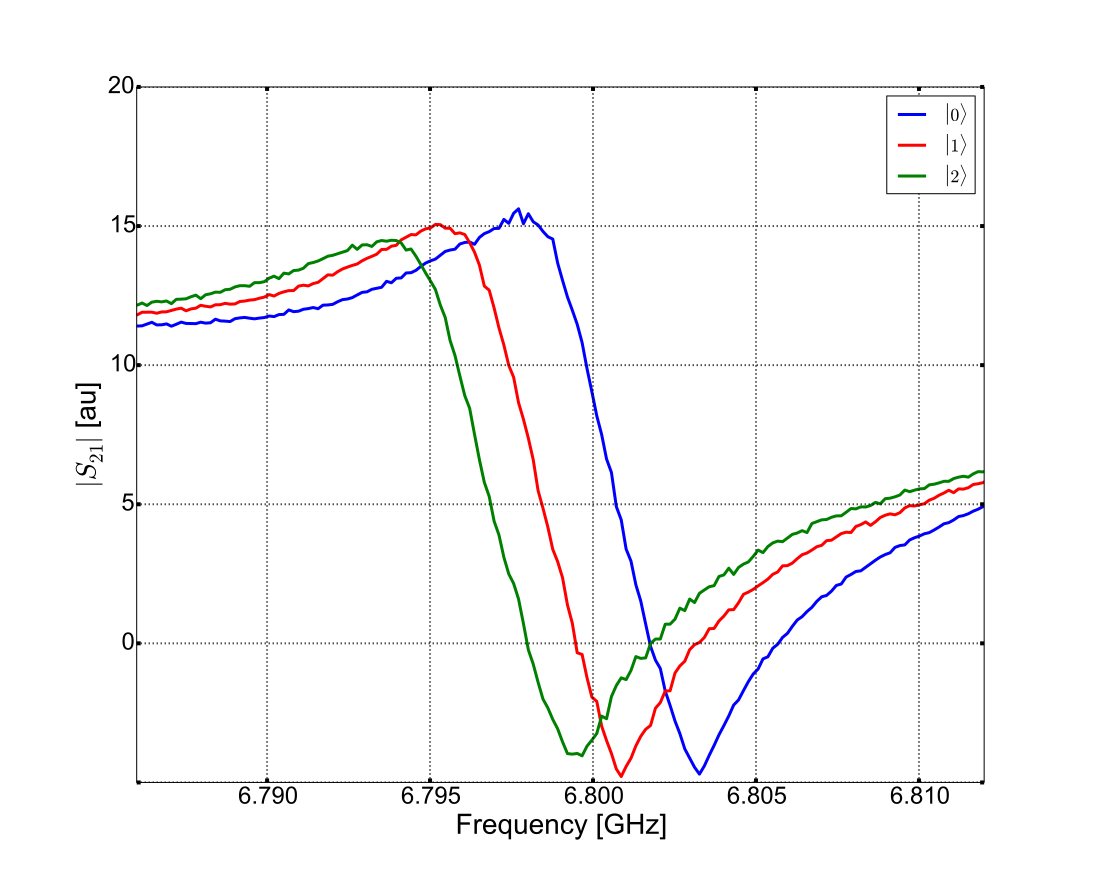
\includegraphics[width=\textwidth]{lollipopDips.pdf}
\par\end{centering}
\caption{Transmission through the measurement circuit for three qubit states. Asymmetry in the resonance dips comes from impedance mismatch in the input and output of the measurement circuit.}
\label{Fig:ch:results:sec:characterization:lollipopDips}
\end{figure}

\begin{table}
\begin{center}
\begin{tabular}{  c  c  c  c  }
\hline \hline
& $\omega_{r}/2\pi$ [GHz]	& \quad $g/2\pi$ [MHz]	& \quad $1/\kappa_{r}$ [ns] \\
\hline
$Q_1$   & \quad 6.835 (6.805)	& \quad 100 (146)	& \quad 19 (12) \\
\hline
$Q_2$   & \quad 6.789 (6.765) 	& \quad 86 (102)	& \quad 37 (23) \\
\hline
$Q_3$   & \quad 6.848 (6.735) 	& \quad 76 (84) 	& \quad 50 (35) \\
\hline
$Q_4$   & \quad 6.737 (6.705)	& \quad 50 (59) 	& \quad 147 (71) \\
\hline \hline
\end{tabular}
\end{center}
\caption{Parameters for the four qubits.  Each was designed with a different target $\kappa_r$ in order to test the tradeoff between damping and measurement speed. Target design values are given in parentheses. Disparity between target and measured values probably comes from errors in predicting in-plane capacitances between structures.}
\label{Table:ch:results:sec:characterization:parameters}
\end{table}


\subsection{Resonator transient response rate - $\kappa_r$}

We next measured the strength of the resonator-environment coupling, characterized by the leakage rates $\kappa_r$.
From the qubit-resonator coupling term in the dispersive Hamiltonian (Eq.\,(\ref{eq:sec:dispersiveHamiltonian:acStark})) we find that the resonator photons shift the qubit frequency by \begin{equation}
\delta \omega_{10} = -2\chi n \label{eq:ch:results:sec:characterization:acStarckShift} \end{equation}
where $n$ is the number of photons in the resonator.
Because the qubit frequency shift is proportional to the photon number, a measurement of the decay time of $\delta \omega_{10}$ yields a measurement of the time decay constant for $n$, which is $\kappa_r$ by definition.

We measured the time decay constant $\kappa_r$ with a ring-down technique.
The pulse sequence is shown in Fig.\,\ref{Fig:ch:results:sec:characterization:photonsVsTime}\,a.
With the qubit in $\ket{0}$ we drive photons into the resonator with a stimulation pulse at the measurement frequency.
During this pulse, photons accumulate in the resonator, raising $n$ and shifting $\omega_{10}$ according to Eq.\,(\ref{eq:ch:results:sec:characterization:acStarckShift}).
The resonator drive pulse is turned off and the resonator is allowed to freely ring down.
As the resonator photon number $n(t)$ changes dynamically during the sequence, the ac Stark shifted qubit frequency also changes as $\delta \omega_{10}(t) = -2\chi n(t)$.
To measure $\omega_{10}(t)$ at each point in time, we apply a $\pi$-pulse to the qubit at variable time $\tau$ and with variable frequency $\omega_{\text{probe}}$.
At each value of $\tau$, the $\pi$-pulse only excites the qubit if $\omega_{\text{probe}} \approx \omega_{10}(t)$.
At the end of the sequence, we measure the qubit state by again probing the resonator, thus measuring the probability that the qubit was excited by the $\pi$-pulse.
This yields a measurement of $\omega_{10}(t)$, as shown in Fig.\,\ref{Fig:ch:results:sec:characterization:photonsVsTime}\,b.
Through Eq.\,(\ref{eq:ch:results:sec:characterization:acStarckShift}) and using the previously measured value of $\chi$, we convert the measured $\omega_{10}$ to $n(t)$, generating a plot of resonator photon occupation versus time during the measurement pulse, as shown in Fig.\,\ref{Fig:ch:results:sec:characterization:photonsVsTime}\,c.
The value of $\kappa_r$ is extracted by fitting the free decay part of the data.
Note that conversion from $\delta \omega_{10}(t) \rightarrow n(t)$ is not necessary for the extraction of $\kappa_r$, as the relevant decay time can be extracted directly from $\omega_{10}(t)$.
We present the $n(t)$ as an accompaniment to the $\delta \omega_{10}(t)$ data shown in Fig.\,\ref{Fig:ch:results:sec:characterization:photonsVsTime}\,b, and because it will be useful later in our discussion of qubit state transitions induced by the measurement photons.

Values of $\kappa_r$ for each resonator are given in Table \ref{Table:ch:results:sec:characterization:parameters}.
The measured values of $\kappa_r$ were approximately 50\% lower than the target values.
This discrepancy has not been understood for our chip.
A subsequent chip using a $\lambda/2$ bandpass filter based on the work described here had a similar error in which the values of $\kappa_r$ were lower than the design values.
It will be important to understand this divergence in the future.

\begin{figure}
\begin{centering}
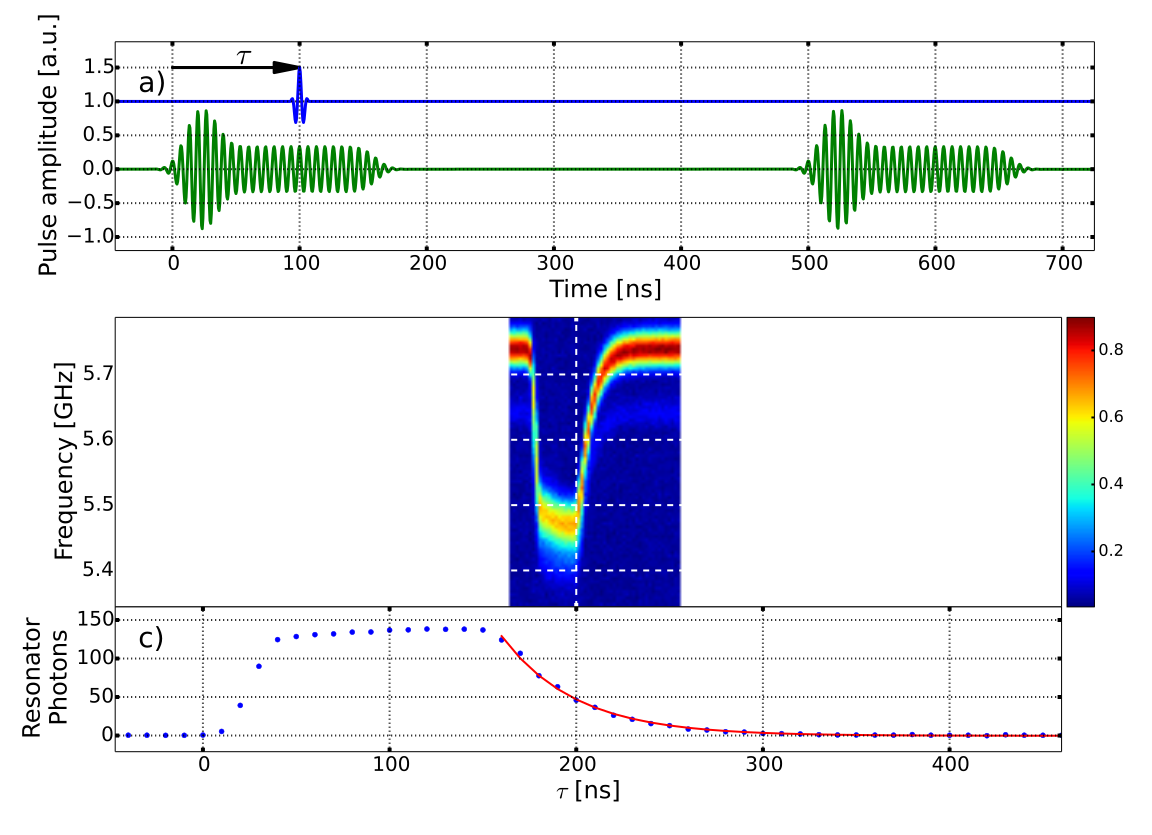
\includegraphics[width=\textwidth]{photonsVsTimeCombined.pdf}
\par\end{centering}
\caption{Resonator photon occupation during the measurement pulse.
a) The control sequence applied to the I port of the IQ mixer used to control the resonator and qubit.
We apply two measurement pulses (green) to the resonator.
Note the emphasis at the beginning of the pulse which acts to ring up the resonator faster than the ring-up time $1/\kappa_r$.
During the first pulse, we apply a $\pi$-pulse (blue) to the qubit at a variable time $\tau$ and frequency.
Only when $\omega_{\text{probe}}$ matches the qubit frequency is the qubit excited.
The second measurement pulse checks whether or not the qubit was excited by the $\pi$-pulse.
b) Probability (color scale) of qubit excitation versus time and frequency of $\pi$-pulse.
The curve of high qubit probability provides a measure of the qubit frequency as a function of time during the measurement pulse.
c) Qubit frequency converted to resonator photon occupation via Eq.\,(\ref{eq:ch:results:sec:characterization:acStarckShift}).
The red curve is an exponential fit to the decay.}
\label{Fig:ch:results:sec:characterization:photonsVsTime}
\end{figure}
